
\chapter{Estado del Arte}


\par Actualmente, el desarrollo y uso de la inteligencia artificial está en boca de todos, pero ¿qué es esta famosa 
inteligencia artificial y por qué ha adquirido tanta relevancia recientemente? A pesar de que ha sido desafiante
definir este concepto durante mucho tiempo, podemos decir que la inteligencia artificial, también conocida 
como inteligencia de máquina (Machine Learning en inglés), es el uso de la inteligencia demostrada por la 
tecnología y maquinas \cite{mt1}. En general, la inteligencia artificial, abreviada como AI (del inglés Artificial Intelligence) 
o IA (de la palabra en español), engloba técnicas como el aprendizaje automático, el aprendizaje profundo y
otros aspectos de la inteligencia artificial \cite{mt1}. Estos temas no son nuevos y han sido objeto de estudio durante 
muchos años. Por ejemplo, en el caso del aprendizaje profundo (Deep Learning en inglés), este se basa en el 
perceptrón, descubierto en 1958 \cite{perceptron}. No fue hasta tiempos recientes, cuando el poder de cómputo y las interfaces 
han sido democratizadas para los usuarios, que hemos podido experimentar y entender realmente lo que la 
inteligencia artificial puede realizar.


\begin{figure}[ht!]
    \centering
    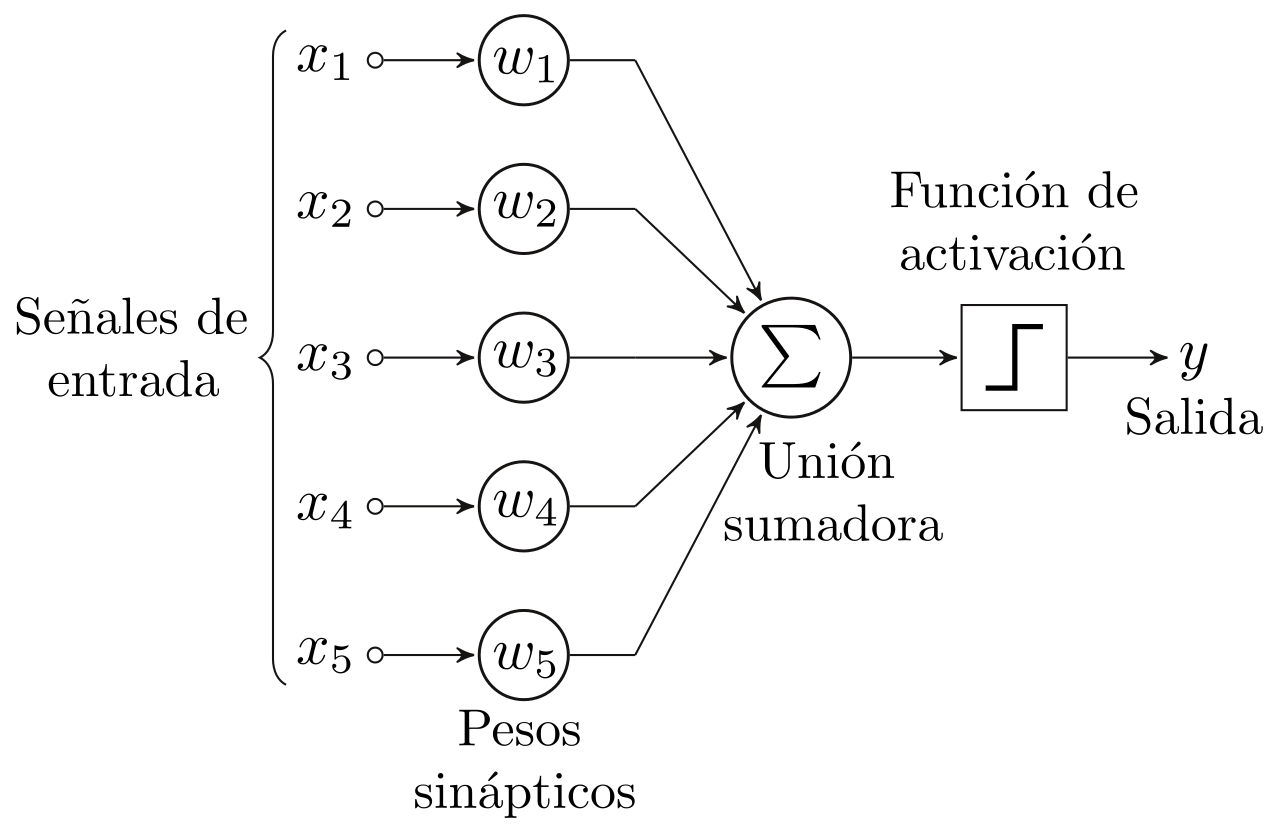
\includegraphics[width=.6\textwidth]{figures/ea1.png}
    \caption[Estructura del perceptrón]{Diagrama de un perceptrón,\\
    {\scriptsize (Fuente: Wikipedia)}}
    \label{fig:ea1}
\end{figure}

\par Luego de entender lo que es la inteligencia artificial ¿Qué es lo diferente que no puede ofrecer actualmente? 
El 30 de noviembre de 2022 es abierto al publico la aplicación ChatGPT por la empresa OpenAI \cite{mt3}, deslumbrando a todos 
con la capacidad de responder las preguntas que le entregaban y con ello elevando aún mas el interés por esta empresa.
La base de esta herramienta nace de una rama especifica de la inteligencia artificial llamada procesamiento del lenguaje 
natural, abreviado NLP, siendo este un subcampo de la Inteligencia Artificial y lingüístico, dedicado a hacer que las 
computadoras comprendan declaraciones o palabras escritas en lenguajes humanos \cite{nlpeda}.


\par El verdaero imparto que provocó ChatGPT en el mundo, fue el conocimiento popular de lo que hoy llamamos inteligencia 
artificial generativa, que puede ser definida como una técnica de inteligencia artificial que genera artefactos sintéticos analizando 
ejemplos de entrenamiento; aprendiendo sus patrones y distribución; y luego creando facsímiles realistas. La inteligencia 
artificial generativa (GAI) utiliza la modelización generativa y los avances en el aprendizaje profundo (DL) para producir 
contenido diverso a gran escala utilizando medios existentes como texto, gráficos, audio y video \cite{mt2}. Por lo que, la población 
general pudo entender que existían herramientas que podían crear y con ello el boom entre la población fue cada vez mas grande. 


\begin{figure}[ht!]
    \centering
    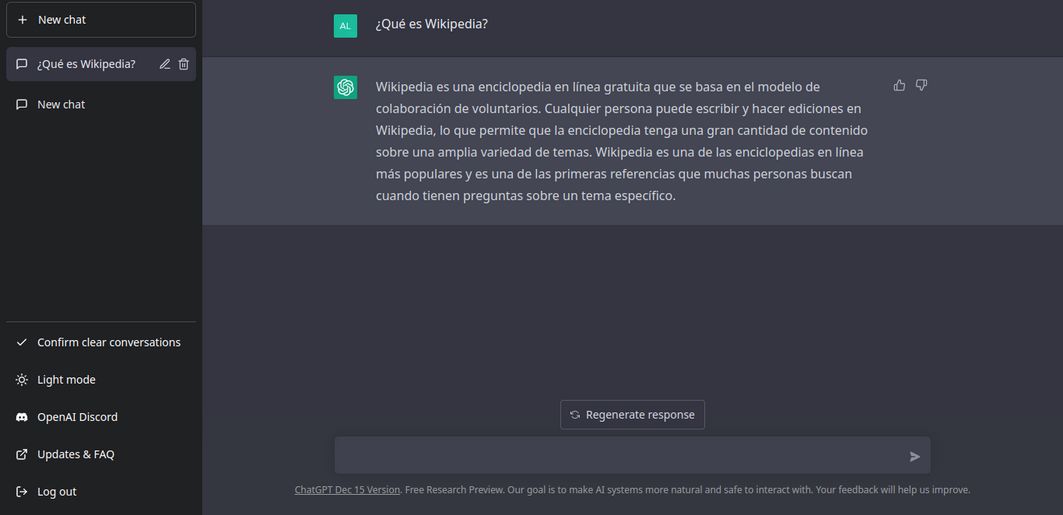
\includegraphics[width=.6\textwidth]{figures/ea2.png}
    \caption[Screenshot de la pagina de ChatGPT]{Screenshot de la pagina de ChatGPT \\
    {\scriptsize (Fuente: ChatGPT)}}

    \label{fig:ea2}
\end{figure}

\par Cuando hablamos de inteligencia artificial y sus aplicaciones, usualmente nos referimos a la generación de modelos. Sin embargo,
en el contexto de la inteligencia artificial generativa, como las herramientas que producen texto o asisten en problemas de 
Procesamiento de Lenguaje Natural (NLP, por sus siglas en inglés), también estamos hablando de un modelo de inteligencia 
artificial. La diferencia radica en que estos son considerablemente más grandes en términos del volumen de datos que manejan. 
Dado que están enfocados en temas de lenguaje, comúnmente los denominamos modelos grandes de lenguaje o LLM, por sus siglas 
en inglés de ``Large Language Models'', siendo estos formalmente definidos como herramientas de inteligencia artificial (AI) 
basadas en redes neuronales recurrentes multicapa que son entrenadas con vastas cantidades de datos para generar texto 
similar al humano \cite{mt6}.

\begin{figure}[ht!]
    \centering
    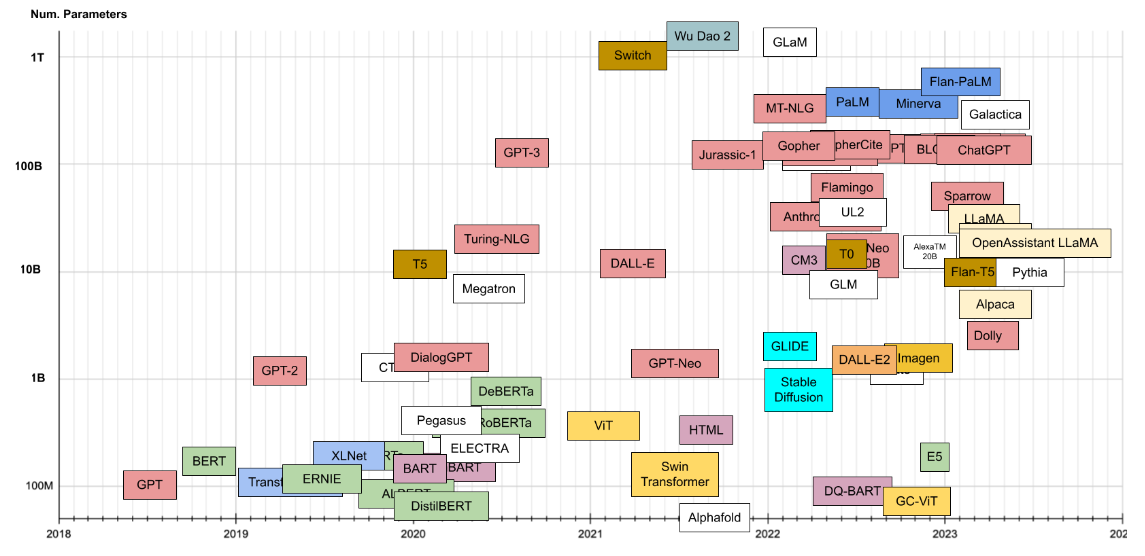
\includegraphics[width=.8\textwidth]{figures/ea4.png}
    \caption[Línea de tiempo del Transformer]{Línea de tiempo del Transformer. En el eje vertical, número de parámetros.
    Los colores describen la familia Transformer,\\
    {\scriptsize (Fuente: Transformer models: an introduction and catalog \cite{eb4})}}

    \label{fig:ea3}
\end{figure}

\par ChatGPT funciona mediante una arquitectura base llamada Transformer \cite{aiayn}, arquitectura creada por Google, que ha generado 
la gran revolución en la inteligencia artificial como la conocemos hasta la fecha debido a que no necesariamente se centra en NLP, 
sino en inteligencia artificial generativa en general. Si somos aún más específicos, GPT viene de Transformer generativo 
pre entrenado, ``Generative Pre-trained Transformer'' en inglés, siendo esta una arquitectura con habilidad de comprender el 
lenguaje de mejor manera usando Transformers \cite{mt4}. Aunque no fue hasta que este modelo creció en la cantidad de parámetros que 
pudo mostrar sus capacidades en la gran amalgama de tareas de procesamiento natural, incluyendo la generación de texto \cite{mt5}.


\begin{figure}[ht!]
    \centering
    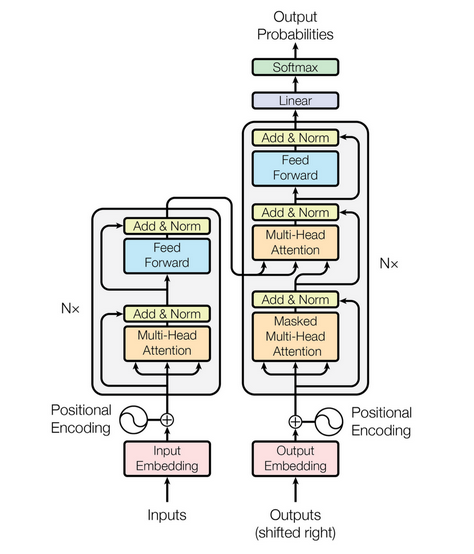
\includegraphics[width=.7\textwidth]{figures/ea3.png}
    \caption[Diagrama de la arquitectura un Transformer]{Diagrama de la arquitectura un Transformer,\\
    {\scriptsize (Fuente: Attention Is All You Need \cite{aiayn})}}
    \label{fig:ea4}
\end{figure}

\newpage

Finalmente, es importante entender el funcionamiento de estos modelos ¿Cómo es posible que logren entender lo que escribo? Los modelos 
GTP funcionan en base a redes neuronales las cuales no entienden ni de letra y palabras, por lo que este texto tiene que pasar por
una función de Embedding. Embedding es el proceso en el que representamos un texto, párrafo o documento de manera numérica, siendo
esta representación en vector de múltiples dimensiones \cite{eb1}, estos vectores se pueden ``grafica'' en un espacio multi dimensional y con 
ello es posible ver la cercanía de cada uno de estos vectores entre ellos, por lo que este vector sirve como punto de entrada para
el funcionamiento de los modelos GTP \cite{eb2}. Ademas, se suelen usar para tareas como busqueda, agrupación, recomendaciones, 
busqueda de anomalias, etc \cite{eb3}.

\begin{figure}[ht!]
    \centering
    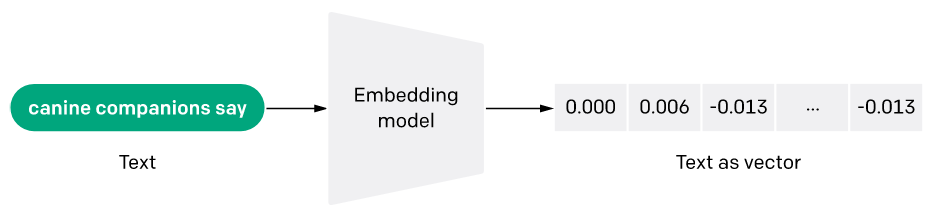
\includegraphics[width=.8\textwidth]{figures/huemul4.png}
    \caption[Diagrama del funcionamiento de un Embedding]{Diagrama del funcionamiento de un Embedding,\\
    {\scriptsize (Fuente: OpenAI\cite{openai1})}}
    \label{fig:ea5}
\end{figure}

